\documentclass[a4paper,11pt]{report}

%\usepackage{a4wide}
\usepackage[english]{babel}
\usepackage{url}
\usepackage[latin1]{inputenc}
%\usepackage[small,bf,hang]{caption2}
\usepackage{xspace}
\usepackage{graphicx}
\usepackage{enumerate}
%\usepackage{fullpage}
%\usepackage[stretch=10]{microtype}
\usepackage{float}
\usepackage{titlesec}
\usepackage{hyperref}
\usepackage{chngcntr}


\counterwithout{figure}{chapter}
\titleformat{\chapter}{\huge\bf}{\thechapter.}{16pt}{\huge\bf}

\begin{document}

\pagenumbering{roman}
\title{Classic\\User Manual}
\author{by Team Classic}
\date{}
\maketitle

\pagenumbering{arabic}
\tableofcontents

\pagebreak
\begingroup
\renewcommand{\clearpage}{}

\chapter{Logging in to Classic}
Browsing to \href{http://student-dp8.intec.ugent.be/}{the Classic homepage} will show you a short introduction of the application. And at the bottom, two buttons can be seen: 'LOGIN' and 'SIGN UP'.

\section{Signing up}
Clicking the 'SIGN UP'-button will bring you to the screen you can see in Figure \ref{fig:sign_up}.

\begin{figure}[H]
\centering
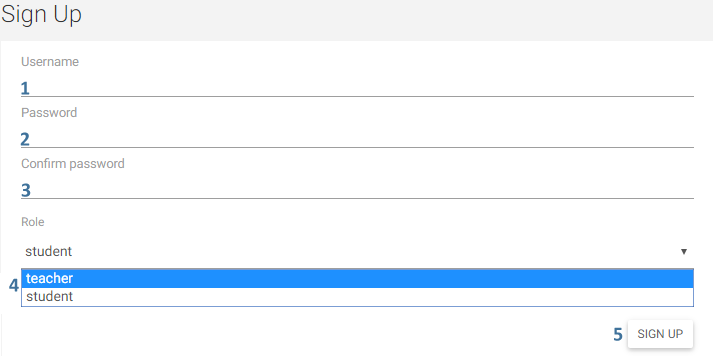
\includegraphics[scale=0.55]{imgs/sign_up.png}
\caption{The 'Sign Up' screen}
\label{fig:sign_up}
\end{figure}
\begin{enumerate}
\item Your username
\item Your password
\item Confirm your password
\item Set the role your account will have, this role dictates what actions you are allowed to do.
\item Clicking the 'SIGN UP'-button will create a new account, if the username is valid.
\end{enumerate}


\section{Logging in}
If you have an account, you can start logging in by clicking the 'LOGIN'-button. Doing so, will show you a screen as shown in Figure \ref{fig:login}.
\begin{figure}[H]
\centering
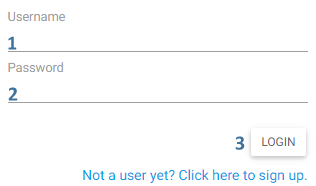
\includegraphics[scale=0.55]{imgs/login.png}
\caption{The 'Login' screen}
\label{fig:login}
\end{figure}
\begin{enumerate}
\item Your username
\item Your password
\item Clicking the 'LOGIN'-button will log your account in, if your password was correct.
\end{enumerate}

\section{Navigation bar}
At all times, you will see a navigation bar at the top of your screen, as shown in Figure \ref{fig:navbar}. This will allow you to go back to a certain point in your Classic browsing history and access your account settings.

\begin{figure}[H]
\centering
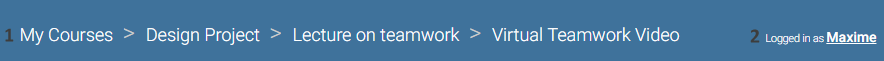
\includegraphics[scale=0.50]{imgs/navbar.png}
\caption{The navigation bar}
\label{fig:navbar}
\end{figure}
\begin{enumerate}
\item Your history; it allows you to go back to 
	\begin{itemize}
		\item All your courses (\textit{My Courses})
		\item The parent course of what you are currently viewing (\textit{Design Project})
		\item The parent lecture of what you are currently viewing (\textit{Lecture on teamwork})
	\end{itemize}
\item Clicking your \underline{name} will bring you to your account-page. For more information, see the account sections under the chapter of your preferred role.
\end{enumerate}


\chapter{Student}
This chapter will guide you through all the actions you are able to do as the role of 'student'. Students are not able to create courses, lectures and cannot add any new files. They can subscribe to courses and watch all the uploaded content. They are also able to add comments and replies to these files.
\section{My Courses}
\label{stu:my_courses}
When you log in, the first thing you see is all the courses you are subscribed to. Figure \ref{fig:stu_my_courses} shows an example of the 'My Courses'-screen of a student that has subscribed to three courses.

\begin{figure}[H]
\centering
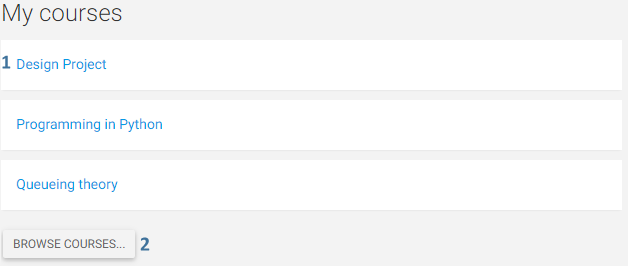
\includegraphics[scale=0.55]{imgs/stu_my_courses.png}
\caption{The first screen you see as you log in, it shows all the courses you are subscribed to.}
\label{fig:stu_my_courses}
\end{figure}
\begin{enumerate}
\item Click on the name of a course to view the contents of this course (see \ref{stu:course}).
\item Click on 'BROWSE COURSES...' to go to the overview of all the available courses (see \ref{stu:browse}).
\end{enumerate}

\subsection{Browse Courses}
\label{stu:browse}
In the 'Course Overview' you can browse all the available courses. Here you can subscribe to new courses and unsubscribe from already subscribed courses, see Figure \ref{fig:stu_course_overview}.

\begin{figure}[H]
\centering
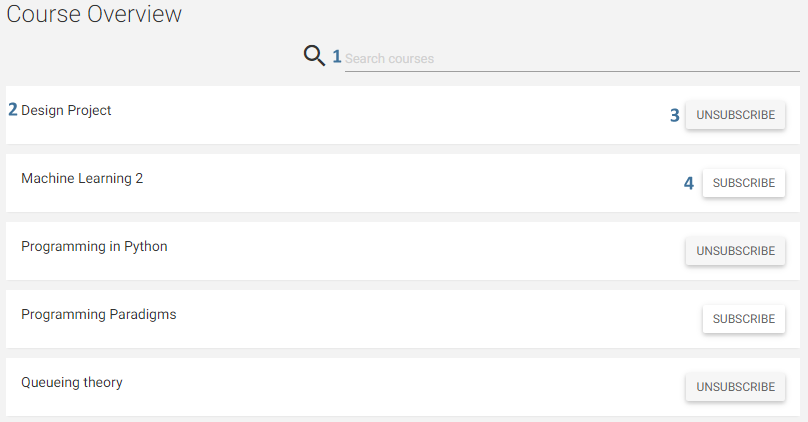
\includegraphics[scale=0.5]{imgs/stu_course_overview.png}
\caption{The overview of all the available courses.}
\label{fig:stu_course_overview}
\end{figure}
\begin{enumerate}
\item Filter the names of courses on your search.
\item The name of a course
\item You can unsubscribe from courses you are already subscribed to.
\item You can subscribe to new courses.
\end{enumerate}


\section{Course}
\label{stu:course}
A student can only view the content of a course. These contents can be \begin{itemize}
\item Lectures
\item Course Videos
\item Course Notes
\end{itemize}

In Figure \ref{fig:stu_course} you see what a course-screen looks like, for a course called 'Programming in Python'.
\begin{figure}[H]
\centering
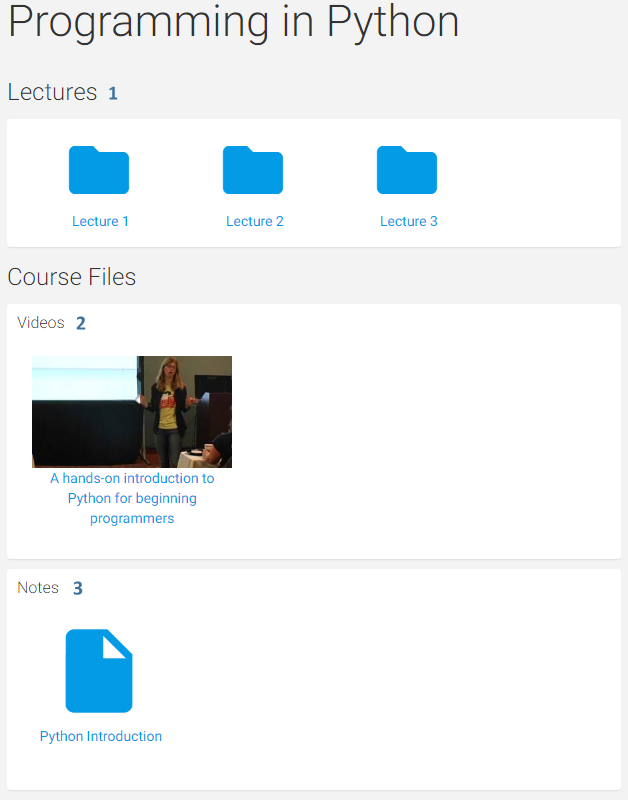
\includegraphics[scale=0.55]{imgs/stu_course.png}
\caption{The page of a course, all the contents can be viewed.}
\label{fig:stu_course}
\end{figure}
\begin{enumerate}
\item All the lectures of this course (see \ref{stu:lecture})
\item All the general videos about this course (see \ref{stu:video})
\item All the general notes about this course (see \ref{stu:notes})
\end{enumerate}


\section{Lecture}
\label{stu:lecture}
A student can only view the content of a lecture. A lecture can only contain videos and notes.

In Figure \ref{fig:stu_lecture} you see what a lecture-screen looks like, for a lecture called 'Lecture 1'.
\begin{figure}[H]
\centering
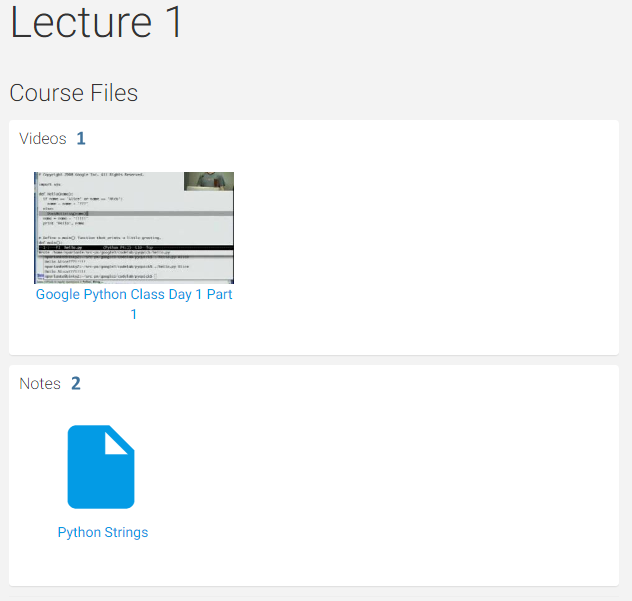
\includegraphics[scale=0.55]{imgs/stu_lecture.png}
\caption{The page of a lecture, you can see the videos and notes.}
\label{fig:stu_lecture}
\end{figure}
\begin{enumerate}
\item All the videos concerning this lecture (see \ref{stu:video})
\item All the notes concerning this lecture (see \ref{stu:notes})
\end{enumerate}

\section{Files}
\label{stu:files}
Under files we understand videos and notes in pdf-form. Comments can be added to both, to videos at a certain point in the video (HH:MM:SS) and to the notes on selected text. So the pages for files are mostly centered around the content of the file and the comment-section.

\subsection{Video}
\label{stu:video}
Videos are shown as seen in Figure \ref{fig:stu_video}, this video is titled \textit{Google Python Class Day 1 Part 1}. On the seek bar (\textbf{1}) you can see yellow cuepoints, these represent comments referring to this point in the video.
\begin{figure}[H]
\centering
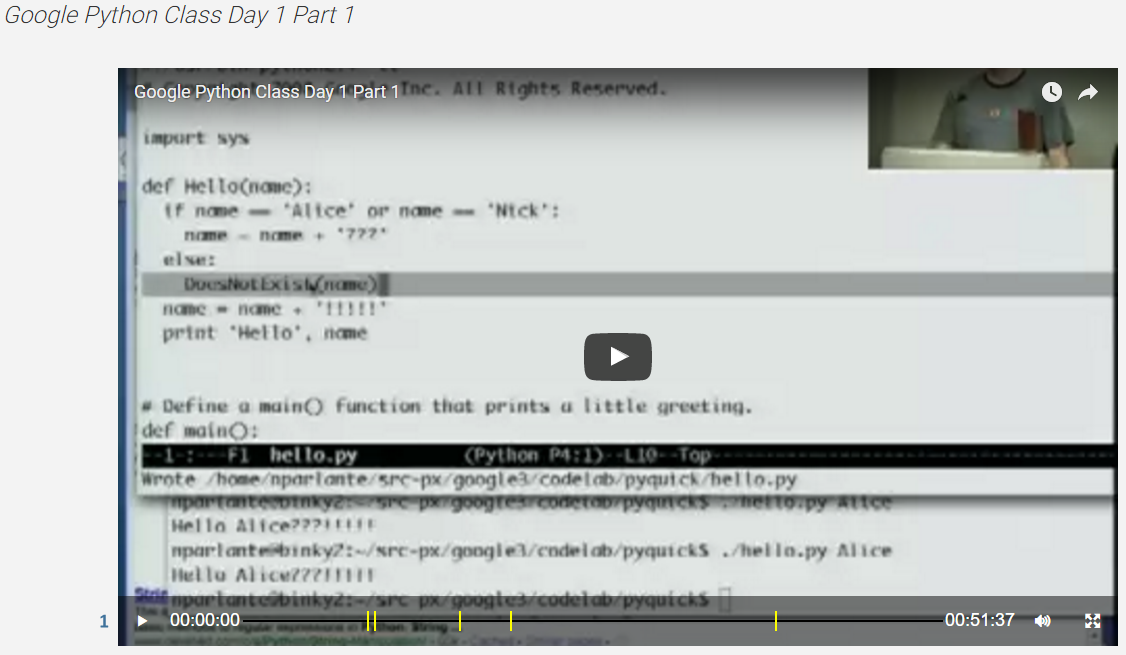
\includegraphics[scale=0.35]{imgs/stu_video.png}
\caption{A video as seen on the Classic platform.}
\label{fig:stu_video}
\end{figure}

\subsection{Notes}
\label{stu:notes}
Notes are shown as seen in Figure \ref{fig:stu_notes}, these notes are titled \textit{Python Strings}. Questions are shown in pink (\textbf{1}) and annotations are shown in orange (\textbf{2}).

\begin{figure}[H]
\centering
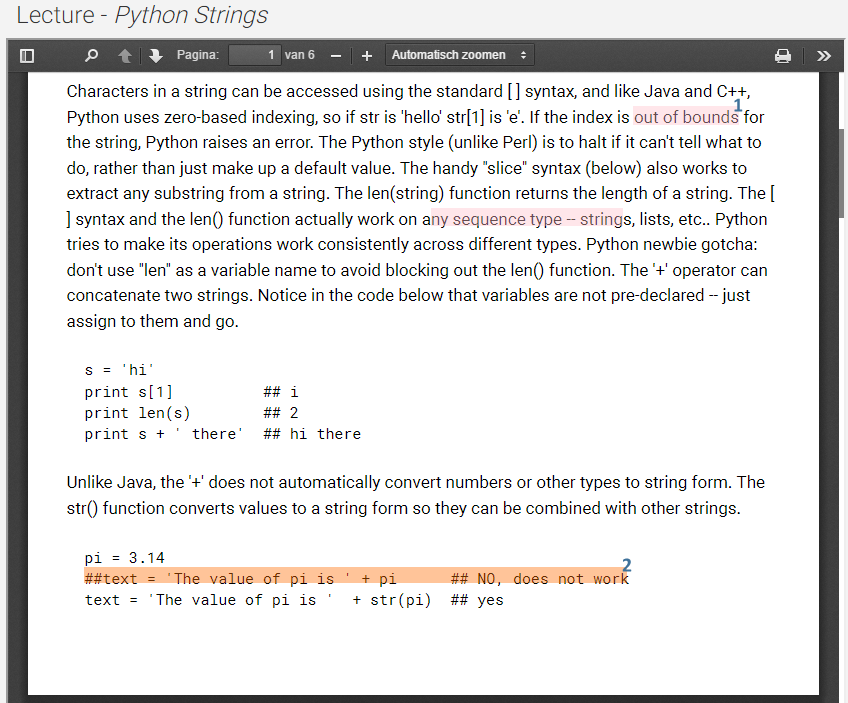
\includegraphics[scale=0.45]{imgs/stu_notes.png}
\caption{Notes as seen on the Classic platform.}
\label{fig:stu_notes}
\end{figure}

\subsection{Comments}
\label{stu:comments}
Although there are a lot of similarities between comments on a video and comments on notes, some things are certainly different. That is why both will be shown and numbered, each number represents an action, but this number may be positioned differently on the video-page than on the notes-page.

\begin{figure}[H]
\centering
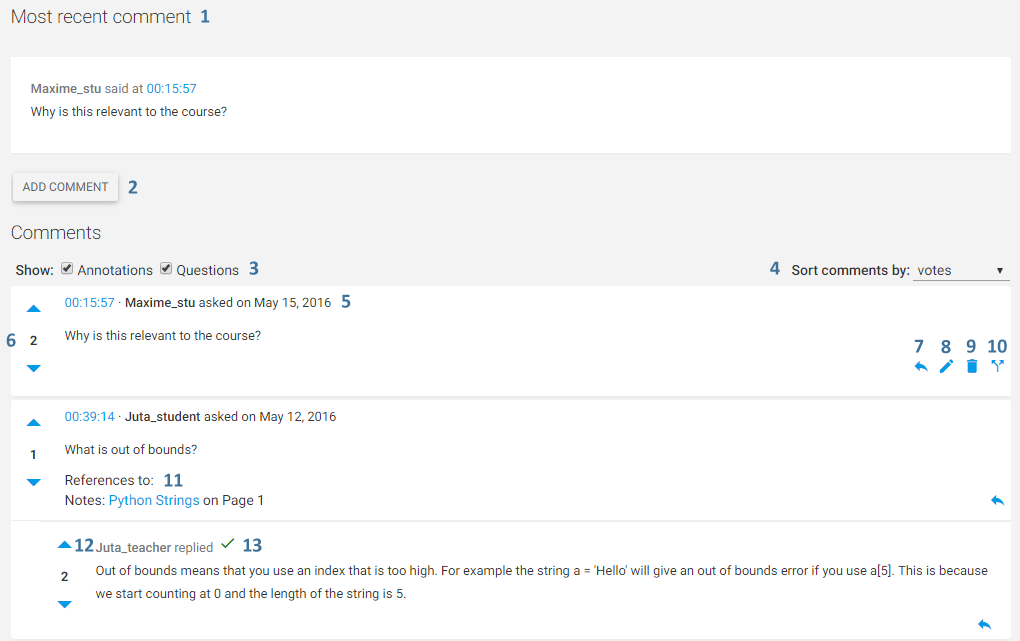
\includegraphics[scale=0.4]{imgs/stu_comments.png}
\caption{Comments on a video as seen on the Classic platform.}
\label{fig:stu_comments}
\end{figure}
\begin{figure}[H]
\centering
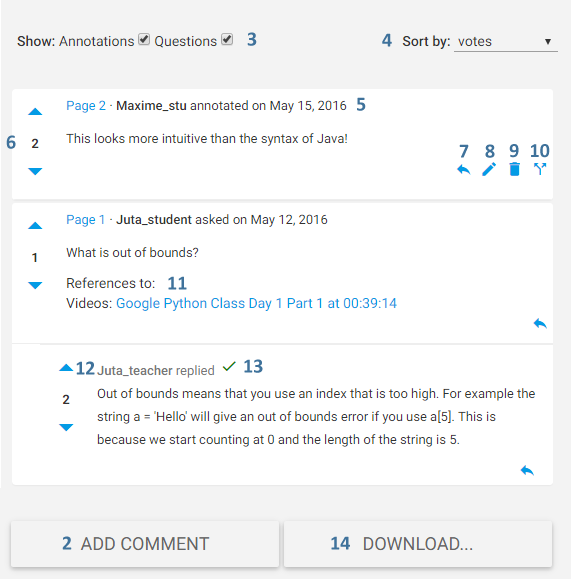
\includegraphics[scale=0.45]{imgs/stu_comments2.png}
\caption{Comments on notes as seen on the Classic platform.}
\label{fig:stu_comments2}
\end{figure}

\begin{enumerate}
\item (\textit{Only seen on videos}) This comment is the most recent comment. It will change when you pass a cuepoint, while watching the video.
\item Clicking this will reveal a form you can fill in to add a comment to this file. See \ref{fig:stu_add_comment} for videos and \ref{fig:stu_add_comment2} for notes.
\item These checkboxes decide what kind of comments are shown, unchecking a checkbox will thus change what comments are shown.
\item This dropdown box enables you to re-sort the comments, based on \textit{votes}, \textit{the date the comment was added} (date) and \textit{where the comment was added to the file} (timestamps or page number). The latter is different for videos and notes. For videos this will be the timestamp the comment was added to, for notes this will be the page number the comment was added to.
\item This is the 'title' of the comment, clicking on the timestamp or page number in front will take you to the position of the file the commented was added. Next is the user and then the date the comment was added. You will also notice that in Figure \ref{fig:stu_comments} it says 'asked', this means that this is a question. In Figure \ref{fig:stu_comments2} it says 'annotated', meaning this is an annotation.
\item Here you see the amount of votes a comment has gotten. Every user can up- and downvote comments, this will influence a comment's positioning when sorting based on votes.
\item Reply to a comment (see Figure \ref{fig:stu_reply}).
\item Edit this comment (see Figure \ref{fig:stu_edit_comment}).
\item Delete this comment.
\item Add a reference to another piece of a file (see \ref{stu:ref}).
\item All the additional references are listed here. In Figure \ref{fig:stu_comments} you can see that a reference to 'Python Strings' is added. While in Figure \ref{fig:stu_comments2} you can see that a reference to 'Google Python Class Day 1 Part 1' was added.
\item This a reply, indicated by the keyword 'replied'.
\item The green check means that this reply has been approved by a teacher or admin.
\item (\textit{Only seen on notes}) Notes can be downloaded to include annotations and/or questions (see \ref{fig:stu_download}).
\end{enumerate}

\begin{figure}[H]
\centering
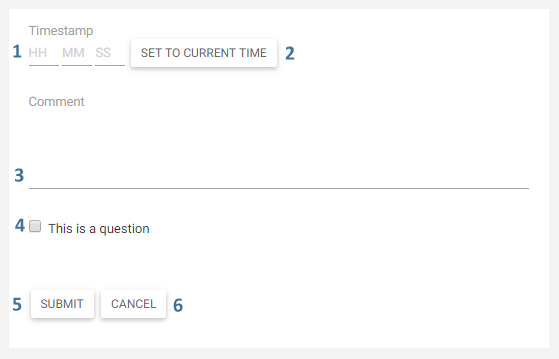
\includegraphics[scale=0.55]{imgs/stu_add_comment.png}
\caption{The form to add a new comment to a video, revealed by clicking 'ADD COMMENT'.}
\label{fig:stu_add_comment}
\end{figure}
\begin{enumerate}
\item Enter a point in time of the video (HH:MM:SS format).
\item Press this button to enter the current time of the video as the timestamp.
\item The body of the comment
\item Check if this comment is a question
\item Click to submit the comment.
\item Click to stop adding a new comment.
\end{enumerate}

The only difference for adding a comment to notes is that instead of giving a timestamp, text must be selected. On \ref{fig:stu_add_comment2} you see that this can be done by selecting the text on the pdf and clicking 'HIGHLIGHT SELECTED TEXT' (\textbf{1}). Another way of doing this is by selecting text on the pdf before clicking add comment, this way the text will be highlighted automatically.

\begin{figure}[H]
\centering
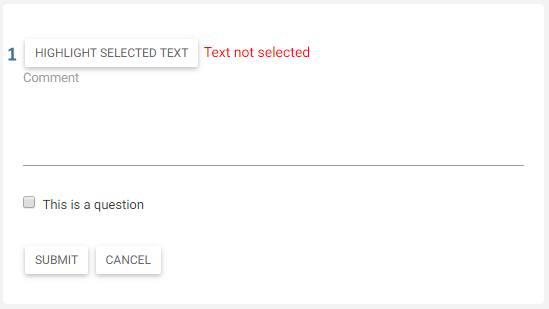
\includegraphics[scale=0.55]{imgs/stu_add_comment2.png}
\caption{The form to add a new comment to notes, revealed by clicking 'ADD COMMENT'.}
\label{fig:stu_add_comment2}
\end{figure}

\begin{figure}[H]
\centering
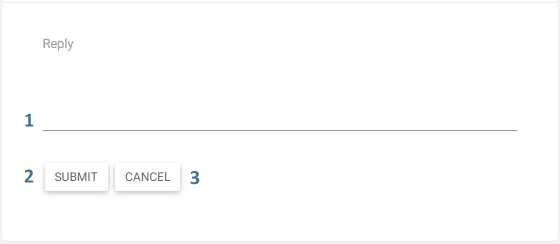
\includegraphics[scale=0.55]{imgs/stu_reply.png}
\caption{The simple reply form.}
\label{fig:stu_reply}
\end{figure}
\begin{enumerate}
\item The body of the reply
\item Click to submit the reply.
\item Click to stop adding a reply.
\end{enumerate}

\begin{figure}[H]
\centering
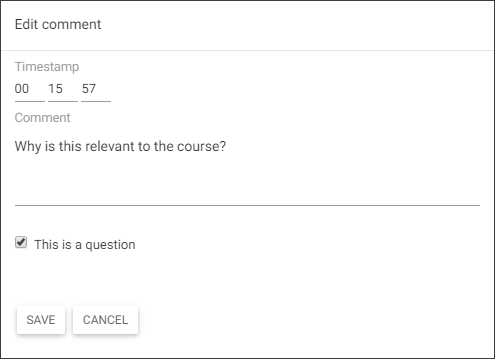
\includegraphics[scale=0.55]{imgs/stu_edit_comment.png}
\caption{The form to edit a comment, the form to edit a reply is similar.}
\label{fig:stu_edit_comment}
\end{figure}
Editing a comment is similar to adding a new comment, but everything is already filled in. Edit what you want to change about the comment and then click 'SAVE' to save your edit.


\begin{figure}[H]
\centering
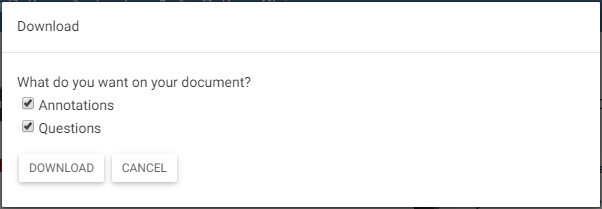
\includegraphics[scale=0.55]{imgs/stu_download.png}
\caption{The choice you get when clicking 'download' on notes, you can choose to include annotations and/or questions in your pdf.}
\label{fig:stu_download}
\end{figure}
Unchecking a checkbox will make it so that those kind of comments are not added to the downloaded pdf. Click 'DOWNLOAD' after the choice is made to start the download in your browser.


\subsection{References}
\label{stu:ref}
Adding additional references (or links) to a comment or reply is what makes Classic so special. By clicking on the two arrows icon on a comment you get to see a form as seen in Figure \ref{fig:stu_ref}.

\begin{figure}[H]
\centering
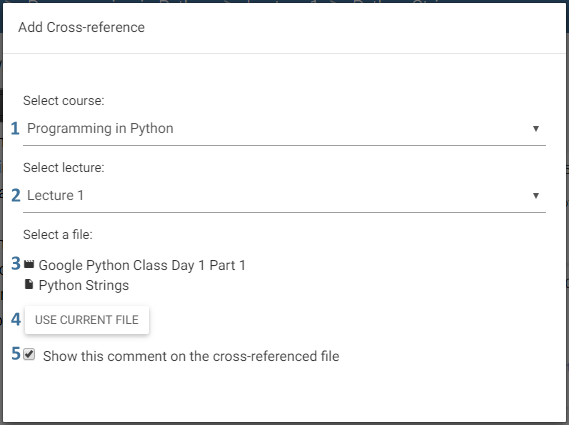
\includegraphics[scale=0.55]{imgs/stu_ref.png}
\caption{The form for adding a new reference to your comment or reply.}
\label{fig:stu_ref}
\end{figure}
\begin{enumerate}
\item Select the course in which the file resides that you want to add a reference to.
\item Select the lecture of the course in which the file resides that you want to add a reference to, you can also choose \textit{no lecture} if you wish to reference a general course file.
\item Finally select the file you want to reference.
\item This is a shortcut if you want to add a reference to the file you are already on.
\item This checkbox decides whether your comment will be seen on the referenced file as well. This is not advised if you are referring to another file for extra information.
\end{enumerate}

Once the file has been chosen, you will get to see the file. Now you have to add a timestamp of the video or select text on the notes, similarly to adding a comment.


\section{Account}
When you click on your \underline{name} in the navigation bar, the account-screen will appear. As you see in Figure \ref{fig:stu_account}, this is where you can view your role.

\begin{figure}[H]
\centering
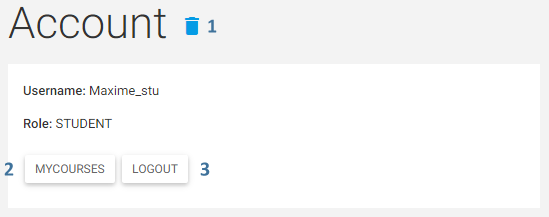
\includegraphics[scale=0.55]{imgs/stu_account.png}
\caption{Your account's settings.}
\label{fig:stu_account}
\end{figure}
\begin{enumerate}
\item Delete this account
\item Go back to 'My Courses' \ref{stu:my_courses}
\item log out from this account.
\end{enumerate}


\chapter{Teacher}
A teacher has the ability to do actions that students cannot, on pages that belong to a course of which the teacher is the owner. Actions such as adding courses, lectures and files and approving comments and replies.

\section{My Courses}
Since a lot is similar on the 'My Courses'-screen, please take a look at \ref{stu:my_courses} first. Figure \ref{fig:tea_my_courses} shows what the screen looks like for a teacher. Notice the \textit{(owner)} tag (\textbf{1}) next to a course of which this teacher is the owner.

\begin{figure}[H]
\centering
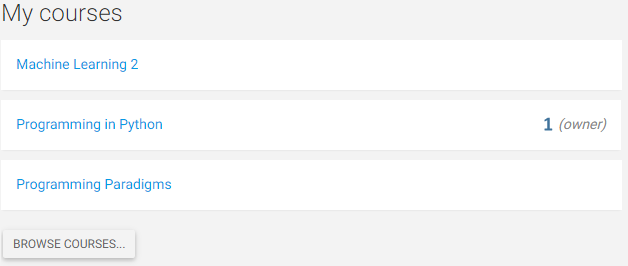
\includegraphics[scale=0.55]{imgs/tea_my_courses.png}
\caption{The first screen you see as you log in, a teacher sees what courses he is the owner of.}
\label{fig:tea_my_courses}
\end{figure}

\subsection{Browse Courses}
When you click on the 'BROWSE COURSES'-button on the 'My Courses'-screen, you still go to the course overview, but here you can now also add new courses (\textbf{1}) and again see the courses of which you are the owner (\textbf{2}).

\begin{figure}[H]
\centering
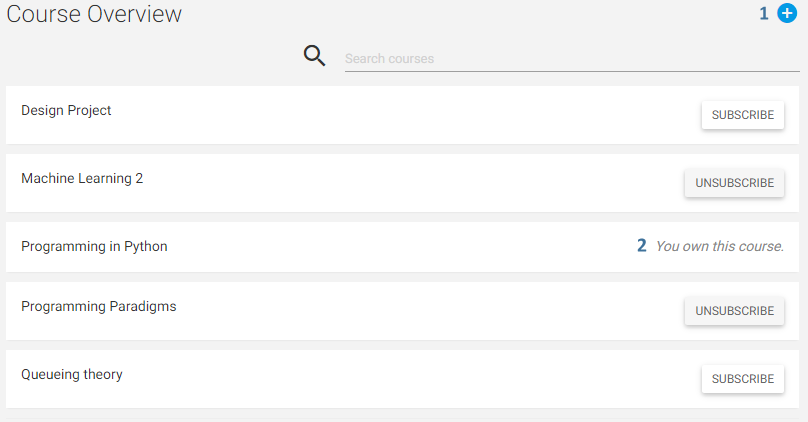
\includegraphics[scale=0.5]{imgs/tea_course_overview.png}
\caption{The overview of all the available courses and the place to add a new course.}
\label{fig:tea_course_overview}
\end{figure}

\section{Course}
\label{tea:course}
For courses of which you are not the owner, this screen is exactly the same as the one students get to see, so see \ref{stu:course} for more information.\\
But if you are the owner of a course, there are a lot more options. You can see in Figure \ref{fig:tea_course} that you can add lectures (\textbf{3}), general videos (\textbf{4}) and general notes (\textbf{5}). A new lecture just needs a name to be added. To add a video, the youtube url should be given before clicking 'ADD'. And lastly adding new notes is done by choosing a local pdf file and clicking 'ADD'.

\begin{figure}[H]
\centering
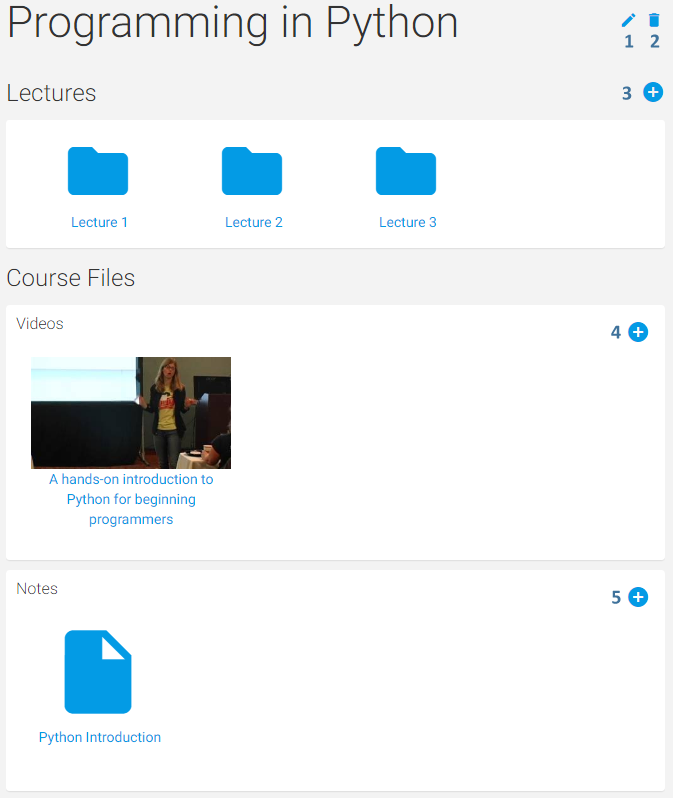
\includegraphics[scale=0.55]{imgs/tea_course.png}
\caption{The page of a course, a teacher can add lectures and files.}
\label{fig:tea_course}
\end{figure}
\begin{enumerate}
\item Go into edit mode. Edit mode allows you to edit the name of the course, by clicking the pencil that appeared next to name of the course. It also allows you to delete lectures and files that belong to this course.
\item delete this course.
\end{enumerate}

\section{Lecture}
When a teacher looks at a lecture of a course he is not the owner of, he sees the exact same as a student (see \ref{stu:lecture}). Similar to courses (\ref{tea:course}), the teacher can go into edit mode (\textbf{1}) and delete the lecture (\textbf{2}). If a teacher is the owner of the course, which the lecture belongs to, he can also add files (\textbf{3} \& \textbf{4}).

\begin{figure}[H]
\centering
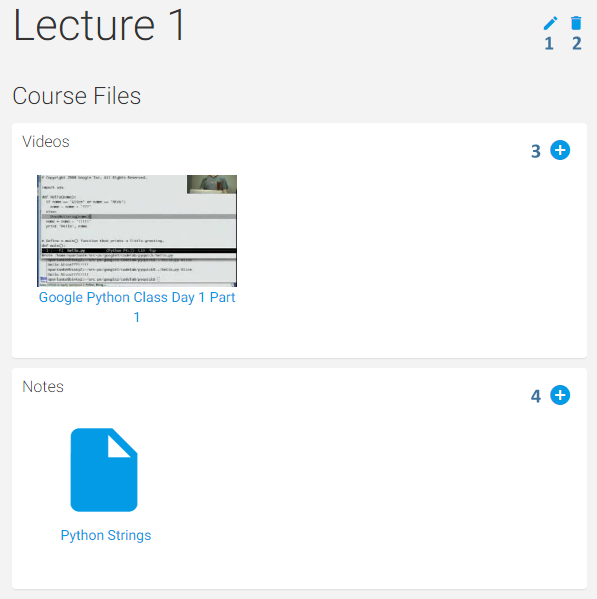
\includegraphics[scale=0.55]{imgs/tea_lecture.png}
\caption{The page of a lecture, a teacher can also add files.}
\label{fig:tea_lecture}
\end{figure}

\section{Files}
Since the file screens are exactly the same, I advice you to check \ref{stu:files} before reading any further. Of course Teachers are able to change the name of files on the file page.\\

In the comments, teachers do have some extra actions in comparison to students. They are able to delete every comment, even if they are not the writer of the comment. The are also able to approve comments by clicking on the 'V' next to trashcan (delete) on a comment. Unapproving is done by clicking on green 'V' next to the title of a comment.

\section{Account}
The account page is exactly the same as it is for students. But the role of your account should of course be 'TEACHER' instead of 'STUDENT'.


\chapter{Admin}
Admins can only be added by contacting an admin, not by signing up on the platform. This is because of the fact that administrators have a lot of rights on the platform. They can do everything a teacher can, as if it is the owner of all courses. Which means he can delete every course, add lectures and files to every course and approve and delete all comments.

\section{Account}

There is one thing that \underline{only} an admin is able to access on the platform. It is found on the account page, as seen in Figure \ref{fig:adm_create_pair}. It is the option to create a new key-secret pair (\textbf{1}) for LTI Single Sign On (SSO).

\begin{figure}[H]
\centering
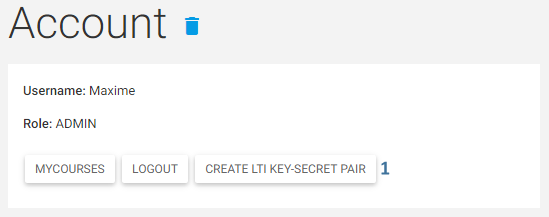
\includegraphics[scale=0.6]{imgs/adm_create_pair.png}
\caption{Your account's settings, as an admin you have an extra button.}
\label{fig:adm_create_pair}
\end{figure}

\begin{figure}[H]
\centering
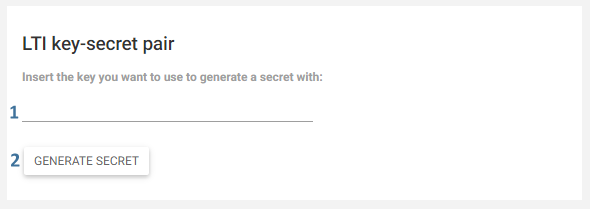
\includegraphics[scale=0.6]{imgs/adm_gen_secret.png}
\caption{The form for generating a new key-secret pair.}
\label{fig:adm_gen_secret}
\end{figure}

In Figure \ref{fig:adm_gen_secret} you see the form for generating a new key-secret pair for LTI SSO.
Enter the key you want to create a secret for (\textbf{1}) and then click on 'GENERATE SECRET' (\textbf{2}) to generate a secret for the given key.\\

After that, you can use this url: \url{http://student-dp8.intec.ugent.be/release/api/lti} as launch url in your LTI consumer platform or application to send POST requests to.

\endgroup
\end{document}